\section{Random Processes}
A \emph{random process} is a function
indexed by a random key.

For example, consider two random
varibles $a$ and $b$ uniformly
distributed in some range. We can define
a function for $-2 \leq 2$
\begin{equation}
    f(t) = at + b
\end{equation}
Then a set of samples from $f(t)$ might
look like

\begin{center}
    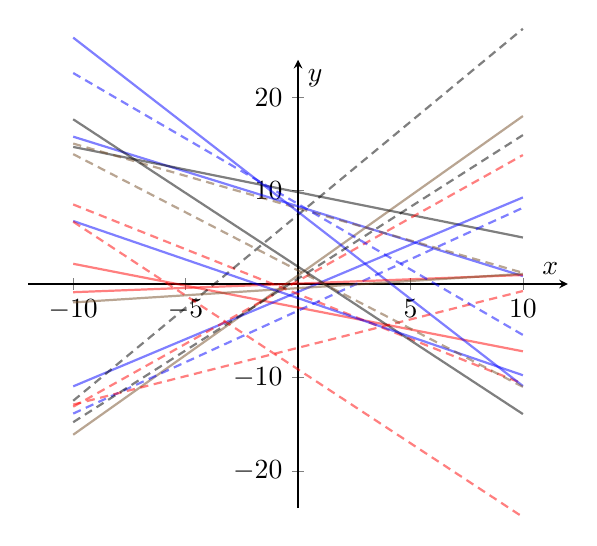
\begin{tikzpicture}
        \begin{axis}[
                xmin=-10, xmax=10,
                ymin=-20, ymax=20,
                axis lines=center,
                samples=2,
                domain=-10:10,
                xlabel=$x$, ylabel=$y$,
                enlargelimits=true,
                clip=false
            ]

            \foreach \i in {1,...,20} {
                    \pgfmathsetmacro{\a}{rnd*4 - 2}
                    \pgfmathsetmacro{\b}{rnd*20 - 10}
                    \addplot+[no marks, thick, opacity=0.5] {(\a)*x + (\b)};
                }

        \end{axis}
    \end{tikzpicture}
\end{center}

This is typically written
\begin{equation}
    f(t, \xi) = a(\xi)t + b(\xi)
\end{equation}
where $t$ is referred to as an \emph{index set}.

We are interested in describing the probability
of obtaining a given set of these lines.

As another example, consider
\begin{equation}
    f(t) = \cos(\omega_0 t + \Theta)
\end{equation}
for $ -1 < t < 1$ where $\Theta$ is
distributed uniformly over the range
$[0, 2\pi]$.

\begin{center}
    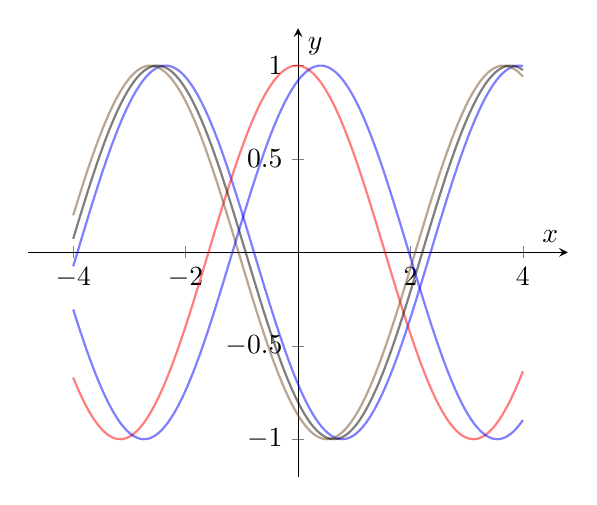
\begin{tikzpicture}
        \begin{axis}[
                xmin=-4, xmax=4,
                ymin=-1, ymax=1,
                axis lines=center,
                samples=200,
                domain=-4:4,
                xlabel=$x$, ylabel=$y$,
                enlargelimits=true,
                clip=false
            ]

            \foreach \i in {1,...,5} {
                    \pgfmathparse{2*pi*rand}
                    \edef\a{\pgfmathresult}
                    \addplot+[no marks, thick, opacity=0.5] {cos(deg((x + (\a)))};
                }

        \end{axis}
    \end{tikzpicture}
\end{center}

Again to be more formal, if $-1 \leq t \leq 1$
and $\xi \in \Omega$,
\begin{equation}
    f(t, \xi) = \cos(\omega_0 t + \Theta(\xi))
\end{equation}

Consider two new kinds of averages, \emph{temporal}
and \emph{statistical}. They are exactly what the names
would imply. To find the temporal average of a random
variable, take one sample and average it over time.
To find the statistical average of a random variable,
average many different samples. The temporal average
gives a random variable, while the statistical average
gives a deterministic function.

For the statistical average, fix a time $t$. We can
look at the 2 dimensional function $X(t, \xi)$ vertically as
\begin{equation}
    \begin{cases}
        X(t, \xi_1) \\
        X(t, \xi_2) \\
        \vdots      \\\
        X(t, \xi_N)
    \end{cases}
\end{equation}
This is a sequence of random variables because
$\xi_1, \dots, \xi_N$ are realizations of the
random variables $\xi$.

For the temporal average, fix the random index
$\xi$. We can look at $X(t, \xi)$ horizontally as
\begin{equation}
    X(t_1, \xi), X(t_2, \xi), \dots, X(t_K, \xi)
\end{equation}
This is a deterministic time series evaluated at
time points $t_1, \dots, t_K$.

The \emph{mean function} $\mu_X(t)$ of a random process
$X(t)$ is
\begin{align}
    \mu_X(t) & = E[X(t)]                             \\
             & = \int_{\Omega} X(t, \xi) p(\xi) d\xi
\end{align}